\chapter{Style Extraction and Transfer}
\minitoc% Creating an actual minitoc

\par We finally arrive to the core objective of the PhD: how to leverage information of style from one (or more) \Gls{task}/s, in order to bootstrap the learning of a new task?


\section{Introduction and objectives}
  % \begin{itemize}
  %     \item Explain different paradigms and metrics used to characterise transfer learning.
  %     \item Why extracting style?: on our side, as ML practitioners, the ultimate objective of using ML is to help us extract new knowledge
  %     \item The questions of research here: extracting styles from bottleneck, transfer between writers, transfer between tasks
  % \end{itemize}

  \par Before we dive into the technical details, it is important to motivate why do we need to perform this in the first place. A common scenario is that we collect data over time for a particular task. This process can be quite expensive (e.g., collecting data from the robots is a slow and expensive process). Then, a new task of interest emerges. This task has common aspects with the old one. The question here is if we can leverage this common aspects, in order to boostrap the learn the new task.

  % For example, in case of handwriting, when trying to write new letters, and need to have the skill of using the pen, and performing micro-actions, like curves and straight lines. In the case of new letters, we need to recombine those mico-actions with new actions, in order to draw the new letters. Another example, in case of humans, is grasping objects. If you learn how to hold a plastic bottle, then you try to hold a glass cup, there are a lot of atomic actions in common, but the forces you apply are different.

  \par Examples of transfer learning:
  \begin{itemize}
      \item If you know how to hold a glass cup, with little adjustments, you can learn how to hold a plastic bottle.
      \item If you know probability and algebra, you can use this knowledge in order to boostrap/accelerate your progress in mastering machine learning.
  \end{itemize}

  \par There are plenty of cases where transfer learning is/could be useful, like:
  \begin{itemize}
    \item In robotics \citep{konidaris2012robot,Konidaris:2012:TRL:2188385.2343689}, collecting data can be quite expensive process, due to hardware limitations from one side, and human limitatio as well (in case of human-robot interaction scenarios). In addition, with techniques like reinforcement learning \citep{sutton2018reinforcement}, where the agent learns by trial and error, the process can be prohibitively slow, with safety concerns sometimes.
    \item In underwater acoustics \citep{malfante2018automatic}, an essential task is collecting and cleaning the data about the different fish sounds. This is a tediously manual job, and any change (type of fish, time of the day or place in the ocean) degrades the quality of prediction a lot. Transfer learning can be very useful in this case, to reduce the effort needed to collect, clean and annotate the data.
  \end{itemize}

  \begin{mdframed}[backgroundcolor=blue!20]
      \begin{center}
          Points addressed in this chapter
      \end{center}

      \begin{itemize}
          \item What is transfer learning? and what are the different approaches to perform it? I will explain the different paradigms and metrics used to characterise transfer learning.
          \item How do we approach the problem of style transfer, for both handwriting and sketch drawing?
          \item The experiments performed, the results, and our conclusions.
      \end{itemize}
  \end{mdframed}

\section{Transfer learning}\label{sec:transfer_learning}
  \par An important research direction in machine learning nowadays is transfer learning. If humans and machines are able to learn how to perform a task, one of the thing that separates humans from machines is the ability to leverage this knowledge in order to acquire new skills and perform new tasks, without the need for additional trials and errors from tabula rasa. This however, is not a straightforward thing for machine learning to do. The algorithms are fitted to data responding directly to the task required (i.e., has the same input feature space and same distribution). Thus, a change in the task can lead to degradation in the algorithm performance \citep{shimodaira2000improving,pan2009survey,weiss2016survey,dtl2018survey}.

  % \par In the following subsections, I first introduced notations and clear description for the objective of transfer learning, and the metrics used to evaluate the quality of transfer. I then discuss different types of transfer learning, with examples on each type.

  % \subsection{Notation and problem definition}
  \par Let's first introduce some notations that will help in formulating the problem:
  \begin{itemize}
      \item We first introduce the concept of \textit{Domain}. A domain defines a feature space (e.g., images of animals), and the probability distribution of this space (i.e., the distribution of pixels in the images of animals). We can consider the domain as the available \textit{knowledge} to us. Thus, a domain $\mathcal{D}$ is defined as $\mathcal{D} = \{\mathcal{X}, P(X)\}$, where:\\
      $\mathcal{X}$ is the feature space, $X$ is the data samples available to us from the feature samples, $X = \{x_1,x_2,\cdots,x_n\} \in \mathcal{X}$, where $n$ is the size of the learning sample. $P(X)$ is the marginal distribution probability of this data sample.

      \item For a given domain (aka, the knowledge available to us), we define a the concept of a \textit{task}. A task is something we would like to achieve using the knowledge we have. For example, a task can be classifying animals given animal pictures, or perform robot navigation given a map of the building. Thus, a task $\mathcal{T}$ is defined as $\mathcal{T} = \{\mathcal{Y}, f(.)\}$, where:\\
      $\mathcal{Y}$ is the label space (the task objectives), $f(.)$ is the mapping function (mapping the domain knowledge to the task objectives). It can also be rewritten as a conditional probability over the domain knowledge, $\mathcal{T} = \{\mathcal{Y}, P(Y|X)\}$.

      % \item Source domain data set, $D_S = \{(x_{1S},y_{1S}),\cdots,(x_{nS},y_{nS})\} = \{X_S,Y_S\}$.\\ Target domain data set, $D_T = \{(x_{1T},y_{1T}),\cdots,(x_{nT},y_{nT})\}= \{X_T,Y_T\}$. Source task $\mathcal{T}_s$, target task $\mathcal{T}_t$.
      \item Based on this notation, we define two more concepts: \textit{Source} and \textit{Target}. A source defines a domain and a task/s that are available to us already (where we have plenty of domain knowledge, and examples on the task/s). A target defines a domain and a task/s as well, where we usually do not have enough domain knowledge and/or examples on the task/s.
  \end{itemize}

  \par Now that we clarified some basic terminology, we can move on to define transfer learning: given source domain data $D_S$, source task $\mathcal{T}_S$,  target domain $D_T$ and target task $\mathcal{T}_T$, we wish to improve the performance of the target task $f_T(.)$ by using $D_S$ and $\mathcal{T}_S$.

  \par Given this definition, we can categorize different types of problems that transfer learning covers:

  \begin{itemize}
      \item The source and taget domains are different, $D_S \neq D_T$, which means that the feature space is different, $\mathcal{X}_S \neq \mathcal{X}_T$, and/or the probability distribution of the feature space are not the same, $P(X_S) \neq P(X_T)$. If $\mathcal{X}_S \neq \mathcal{X}_T$, the transfer learning problem is \textit{Heterogeneous}. Otherwise, it is \textit{Homogeneous}.

      \item The source and target tasks are different, $\mathcal{T}_S \neq \mathcal{T}_T$, which means that the objectives are different, $\mathcal{Y_S} \neq \mathcal{Y_T}$, and/or the mapping function (from the feature space to the objectives) are different, $P(Y_S|X_S) \neq P(Y_T|X_T)$.
  \end{itemize}

  % \par Many approaches in order to achieve transfer learning has been proposed in the literature. We will discuss the different approaches, and give examples from the literature on each one. We follow the categorization of transfer learning approaches done in \citep{weiss2016survey}, by first identifying two main categories of transfer learning:
  % \begin{itemize}
  %   \item \textit{Symmetric} feature transformation attempts to discover underlying meaningful structure between domains, to find common latent features that unify (or at least reduce) the marginal distribution of the two domains.
  %
  %   \item \textit{Asymmetric} feature transformation attempts to transfer the features of the source space to make them more closely match the target space. See figure \ref{fig:feature_transformation}.
  % \end{itemize}
  \par Many approaches in order to achieve transfer learning has been proposed in the literature. We will discuss the different approaches, and give examples from the literature on each one. We follow the categorization of transfer learning approaches done in \citep{dtl2018survey}\endnote{Other categorization exists, like the one used in \citep{weiss2016survey}. When it comes to deep transfer learning, we believe the one in \citep{dtl2018survey} to be the most relevant.}, by first identifying two main categories of transfer learning:
  \begin{itemize}
    \item \textit{Instances-based}: in this case, we utilize examples from the source domain into the training of the new target domain, by defining weights on them.
    \item \textit{Mapping-based}: the objective in this case is to project the instances from the two domains into a new manifold, that increases the similarity between the two domains.
    \item \textit{Network-based}: the more common type of deep transfer learning. It is based on the idea that the layers of the deep neural network extracts basic and general information, that shared a lot with other domains. In this case, the network or some of its layers are re-used on the target task.
    \item \textit{Adversarial-based}: using generative adversarial networks \citep{goodfellow2014generative} in order to find a manifold that are fit for both source and the target domains.
  \end{itemize}

  % \begin{figure}[!htbp]
  % \centering
  % 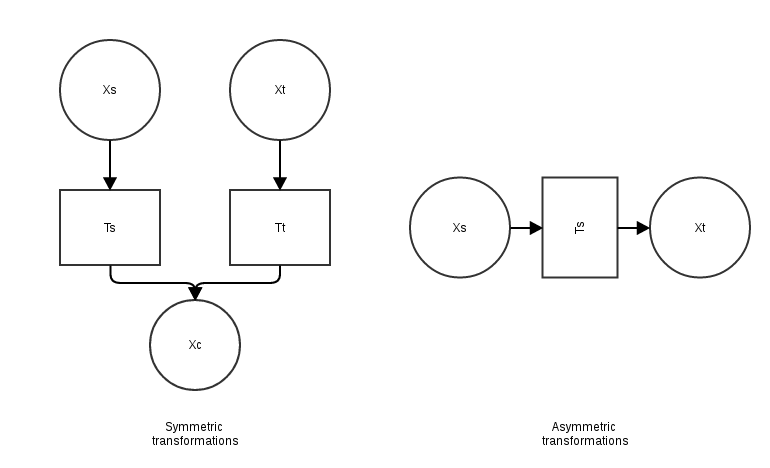
\includegraphics[scale=0.4]{images/sota/feature_transformation.png}
  % \caption[Symmetric and Asymmetric transfer]{Illustration for the difference between Symmetric and Asymmetric feature transformation \textbf{REDO THE DIAGRAMS -- NOT CLEAR}}
  % \label{fig:feature_transformation}
  % \end{figure}

  % Note: I no longer see that this section is relevant. These metrics make sense in RL domain, not in
  % \subsection{Metrics to evaluate transfer learning}
  % \par There is no one way to evaluate transfer learning; it depends on the needed requirements. Several metrics have been proposed in the literature \citep{taylor2007cross}, like (see also figure \ref{fig:tl_metrics}) \GB{complete figure to have these 4 features}:
  % \begin{enumerate}
  %     \item Jump start: It is the difference in the initial performance between using transfer relative to learning without transfer.
  %     \item Asymptotic performance: The difference in the learning performance through time/epochs between using transfer relative to learning without transfer.
  %     \item Total Reward/Accuracy difference between end-performance with vs. without transfer learning.
  %     \item Time-to-threshold: It the amount of time (or number of samples) needed to achieve a pre-specific performance level.
  % \end{enumerate}
  %
  % \begin{figure}[!htbp]
  % \centering
  % 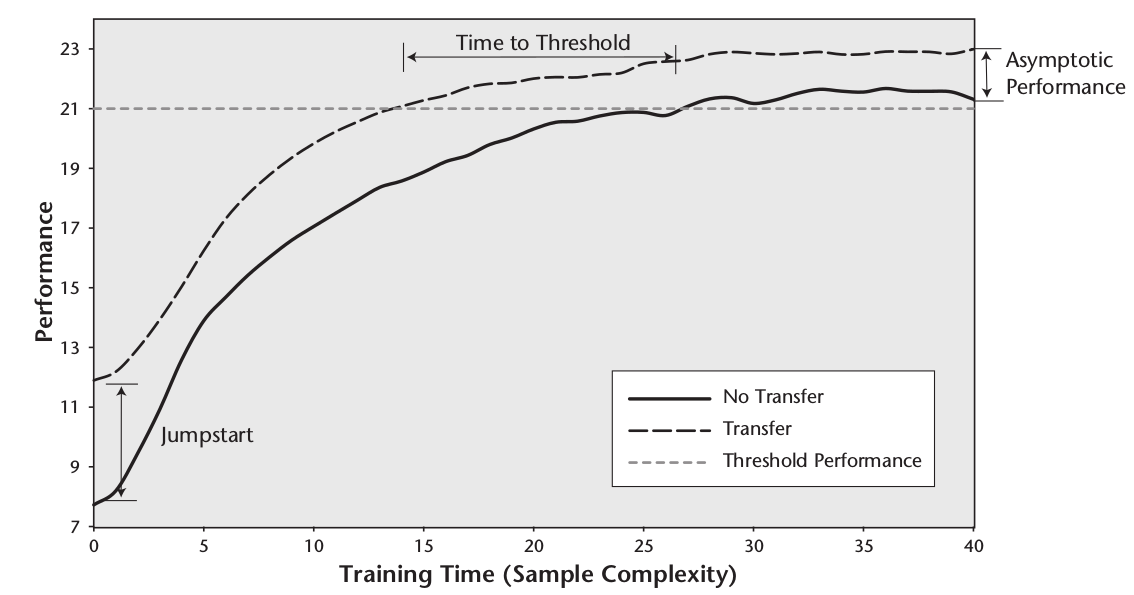
\includegraphics[scale=0.3]{images/sota/TL_metrics.png}
  % \caption{Different proposed metrics to measure transfer learning \textbf{Mention the source of this image}}
  % \label{fig:tl_metrics}
  % \end{figure}
  %
  % \par The transfer is considered as successful if metric 1 is greater than zero, metrics 2-3 increases with transfer or metric 4 reduces through transfer. It is worth mentioning that, in most state of the art, only metrics 3 and/or \GB{4??} are reported (which are the relevant metrics in my opinion for our work). I report all those metrics however, since I believe they give us a good diagnostics for our transfer learning system.

  % New try to attack this problem

  \par When it comes to evaluating the success of the transfer, there is no one way to evaluate transfer learning in general. This depends a lot on the objectives of transfer learning, and the criteria of success. In the case of machine learning, the improve in end quality of the model is the primary performance aspect being measured and reported -- like the classification accuracy \citep{chattopadhyay2012multisource,long2013transfer,pan2010cross,glorot2011domain}, the reduction in the average error \citep{pan2010domain}, ...etc --. The transfer is considered successful if it achieves better performance to the baseline method.

  \par We expect that, with the introduction of transfer learning via deep learning, that the \textit{time to train} the model could be another aspect to consider -- similar to what is being done in reinforcement learning \citep{taylor2007cross} --, although -- to the best of our knowledge -- we do not find studies mentioning this at the moment.

  \subsection{Homogeneous transfer learning}
  \par In this case, most of the research are focused on one of the 3 areas:
  \begin{itemize}
      \item Correct for source marginal distribution $P(X_S)$, to make it more alligned with the task marginal distribution $P(X_T)$.
      \item Correct for the source mapping function (between the domain knowledge and the task), $P(Y_S|X_S)$, to make it more alligned with the target mapping function, $P(Y_T|X_T)$
      \item Both.
  \end{itemize}

  \subsubsection{Symmetric - transfer learning using deep learning}
  \par \citep{glorot2011domain} discusses a deep learning approach for transfer learning for sentiment classification, by using stacked de-noising auto-encoders \citep{vincent2008extracting} to correct the marginal distribution between the source and the target domain, by learning latent variables/features common between the two data sources in two steps:
  \begin{itemize}
      \item First, train an auto-encoder on the unlabeled data from the source and the target. This will produce latent variables that will make $P(X_S)$ closer to $P(X_T)$.
      \item Use those latent features to train a classifier on the labeled source data.
  \end{itemize}
  \par Experiments are done on 12 different sources and target domain pairs. The data used reviews for different products (4 different products). The performance metric used in this case is the classification error rate when using a classifier trained on the source task only, minus the classification error rate of a classifier trained on the target task only. A SVM classifier trained on the source domain is used as a baseline, and a comparison with other transfer methods \citep{blitzer2006domain,li2008multi,pan2010cross}. All these methods performs better than the baseline, and \citep{glorot2011domain} peforms better than all of them.

  \par \citep{malfante2018use} compares the use of deep transfer learning to manual features \citep{malfante2016automatic,malfante2018machine}, in order to recognize the sounds of fish underwater. Interestingly, the deep learning models are trained on ImageNet \citep{imagenet_cvpr09} dataset (which is completely unrelated to acoustics), then used in order to extract features from the spectrogram of the underwater recordings. The assumption here is the the filters learned with deep learning are basic and generic enough, to be used in other domains, thus, deep learning can provide a natural correction for $P(X_S)$, to make it close to $P(X_T)$. Without any finetuning, the deep learning achieves quite a high perfomance, although less than the state of the art, suggesting that a further investment in this direction is worth the time.

  \par The idea of using deep learning~\citep{lecun2015deep} in order to achieve transfer learning has gain popularity during the last years, following the achievements in having better computational resources~\citep{raina2009large}, and the availability of large benchmark datasets - most notably: ImageNet~\citep{imagenet_cvpr09} for object detection, MS-COCO~\citep{2014arXiv1405.0312L} for image captioning~\ldots
  \GB{Give general/key idea rapidly: pre-training of feature extractions performed by layers close to input, vs. training of high-level processing performed by layers close to output.}

  \par The first notable success of deep learning happened in the area of computer vision, with the AlexNet architecture~\citep{krizhevsky2012imagenet}. It was found out that such a deep network manages to extract generic features about the images: it learns simple, hierarchical filters, that are generic enough to be applicable for different datasets (see figure~\ref{fig:AlexNet_filters}). This observation led to another surge in the usage of pretrained AlexNet - and later newer architectures, like VGG16~\citep{simonyan2014very}, Inception~\citep{szegedy2015going},etc - as feature extractors for new, unseen datasets.

  \begin{figure}[!htbp]
  \centering
  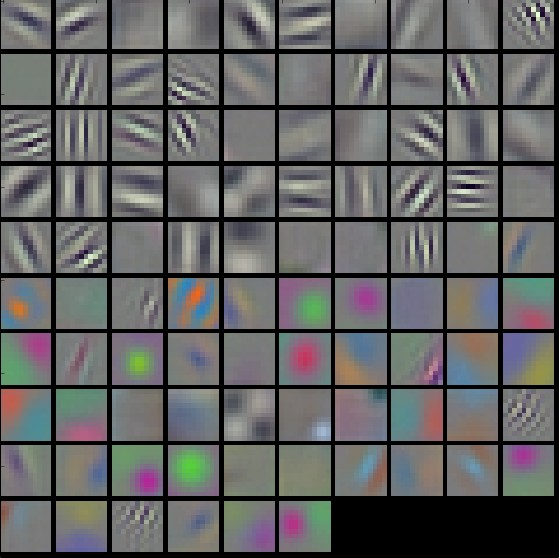
\includegraphics[scale=0.4]{images/sota/filt1.jpeg}
  % \caption{Visualization of the first convolution layer of a trained AlexNet. The weights are very nice and smooth, indicating nicely converged network. Note also the basic simple shape of filters. It easy to imagine that those same filters will be useful in other computer vision or image related tasks.}
  \caption[Convolution Neural Networks filters shape]{Visualization of the first convolution layer of a trained AlexNet. Note the basic shape of filters that resemble to Gabor filters widely used in image processing for decades~\citep{fogel1989gabor,jain1991unsupervised}. It easy to imagine that those same filters will be useful in other computer vision or image-related tasks.}
  \label{fig:AlexNet_filters}
  \end{figure}

  \par It is interesting to note that those filters can be also seen as a representation for the skills we want to extract. In our case, we will need to combine both deep convolution network with a recurrent neural network (like in \citep{s16010115,pinheiro2014recurrent,huang2016deep}).

  \subsubsection{Parameter-based transfer}
  \citep{chattopadhyay2012multisource} propose a conditional probability based domain adaptation (CP-MDA): it corrects the difference between conditional probability distributions of multiple labeled source data, vs. limited amount of labeled target data. The process has five main steps:
  \begin{enumerate}
      \item Build a classifier for each of the source domains
      \item Measure the closeness of each of those classifiers to the conditional distribution of the target domain.
  %(NOTE: I don't understand yet how it is done).
      \item Weight the classifiers according to their closeness
      \item Use the weighted source classifiers to find pseudo labels for the unlabeled target data
      \item Train a new classifier to map between the pseudo labels and the real labels on the targets data
  \end{enumerate}
  Experiments are done on fatigue classification (surface electromyography data). Different source domain is for different people.

  \subsubsection{Instance-based transfer}
  \citep{chattopadhyay2012multisource} developed a weighting framework for multi-source domain adaptation (2SW-MDA). It tries to correct both the marginal and the conditional distributions between the source and the target domains in three steps:
  \begin{enumerate}
      \item Weight each source domain based on the marginal distribution difference between it and the target domain
      \item Source domain weights are updated according to the (CP-MDA) approach
      \item The target classifier is learned based on the re-weighted source classifiers and the labelled target data.
  \end{enumerate}
  %(NOTE: To be review again how this learning happens)
  Experiments are done on fatigue classification (surface electromyography data). Different source domain is for different people.

  % \subsection{Relational based transfer}
  % \subsection{Hybrid based transfer}

  \subsection{Heterogeneous transfer learning}
  \par In this case, most of the research are focused on only one area: Aligning $\mathcal{X_S}$ with $\mathcal{X_T}$, assuming that $P(X_S) = P(X_T)$.

  \subsubsection{Symmetric}
  \citep{shi2010transfer} developed a method called \emph{Heterogeneous Spectral Mapping} (HeMap). It is assumed that: $\mathcal{X_S} \neq \mathcal{X_T}$, $P(X_S) \neq P(X_T)$ and $\mathcal{Y_S} \neq \mathcal{Y_T}$. It also assumes the availability of labeled source data, and limited labeled target data.
  \begin{itemize}
      \item First is to find common latent variables between the source and the target domains, by using spectral mapping techniques. The spectral mapping objective is to maintain the original data structure, while minimizing the difference between the two domains (NOTE: Review the way it is formalized).
      \item Second, a cluster based sampling is performed to selected new training data (Thus, correcting the difference in marginal distribution).
      \item Third, correct the conditional distribution by Bayesian methods (NOTE: To be reviewed again, not clear to me).
  \end{itemize}
  Experiments are performed on image classification and drug efficacy prediction. (NOTE: The results are not clear, as they don't mention what is the baseline exactly, and no comparison to other state of the art methods is performed).

  \subsubsection{Asymmetric}
  \citep{Nam:2015:HDP:2786805.2786814} discuss the application of transfer learning in software module defect problem. The source and the target software projects collect different performance metrics. The solution developed is called heterogeneous defect prediction (HDP). \endnote{This solution performs well on the assumption that the source and the target features are statistically close}.
  \begin{itemize}
      \item First, perform feature selection on the source and on the target data, in reduce the dimensionality.
      \item Second, a statistical comparison (Kolmogorov-Smirnov test) is performed between the reduced source and target features, in order to determine the closeness of different features.
      \item Third, train a classifier using those close source features.
      \item Fourth, use this classifier on the target data, where the input will be the corresponding target features (related to the source features from the previous step).
  \end{itemize}

  \subsection{Negative transfer}
  \par A concern that arises in transfer learning is what is called \textit{negative transfer}, where the knowledge learned from one task leads to no improvement on the target task, but reduces the quality of learning for that task. This can happen for multiple reasons, for example:
  \begin{itemize}
      \item The source task is not sufficiently related to the target task, thus, in the best case scenario, no useful knowledge can be transferred.
      \item The transfer method is not able to exploit the similarities between the source and the target task
  \end{itemize}
  Within the framework of \textit{reinforcement learning}, some methods can estimate task similarity \citep{taylor2008transferring, torrey2010transfer}, though these methods do not provide any theoretical guarantees about their effectiveness. This, however, is an open area of investigation in the framework of \textit{supervised learning} \textbf{CAN'T FIND RESOURCES HERE}. The main thing here for us to be careful during the choice/design of the source and the target experiments, to ensure that a possible positive transfer learning can happen.

\section{Application of transfer learning}
  \par In the previous section, we explored the concept of transfer learning, and the different categories mentioned in the literature about this
  In the section, I will explain the work done during the PhD on transfer learning. There are two questions we addressed:
  \begin{itemize}
      \item Transfer between writers
      \item Transfer between tasks
  \end{itemize}

  \subsection{Transfer between writers}
  \subsection{Transfer between tasks}

    \subsubsection{IRONOFF}
    \subsubsection{QuickDraw!}
      \begin{figure}
        \centering
        \begin{subfigure}[tb]{0.45\textwidth}
            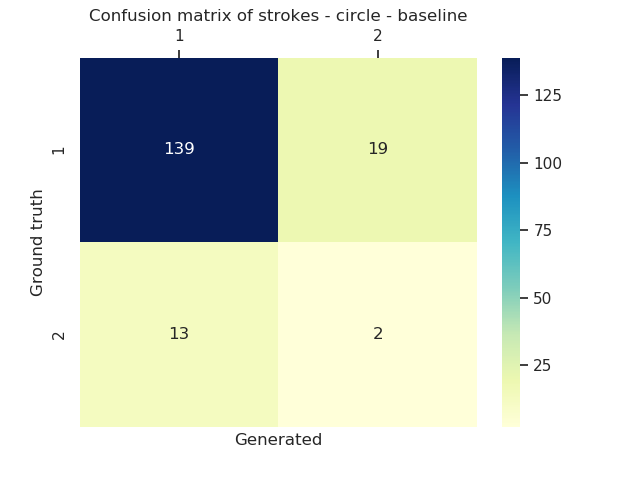
\includegraphics[width=\textwidth]{images/sota/quickdraw_results/quickdraw_circle_target_strokes_heatmap.png}
        \end{subfigure}
        ~
        \begin{subfigure}[tb]{0.45\textwidth}
            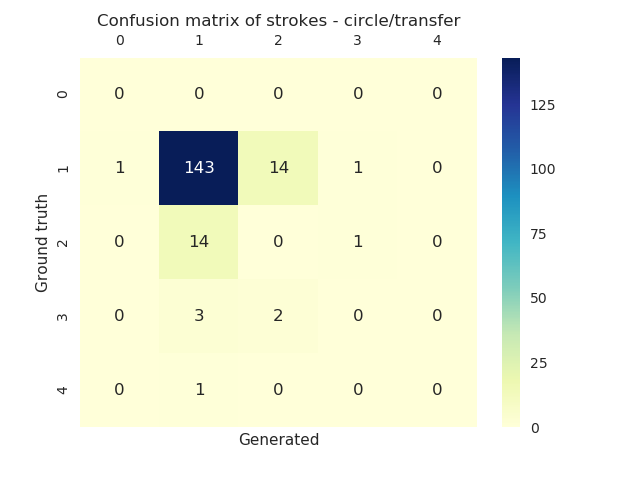
\includegraphics[width=\textwidth]{images/sota/quickdraw_results/quickdraw_circle_transfer_strokes_heatmap.png}
        \end{subfigure}

        ~
        \begin{subfigure}[tb]{0.45\textwidth}
            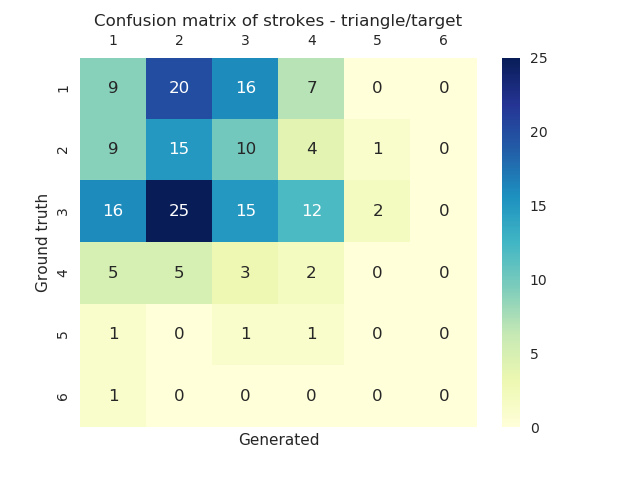
\includegraphics[width=\textwidth]{images/sota/quickdraw_results/quickdraw_triangle_target_strokes_heatmap.png}
        \end{subfigure}
        ~
        \begin{subfigure}[tb]{0.45\textwidth}
            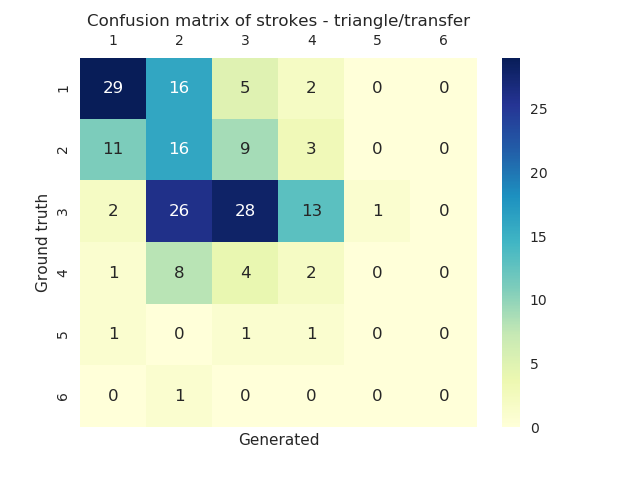
\includegraphics[width=\textwidth]{images/sota/quickdraw_results/quickdraw_triangle_transfer_strokes_heatmap.png}
        \end{subfigure}

        ~
        \begin{subfigure}[tb]{0.45\textwidth}
            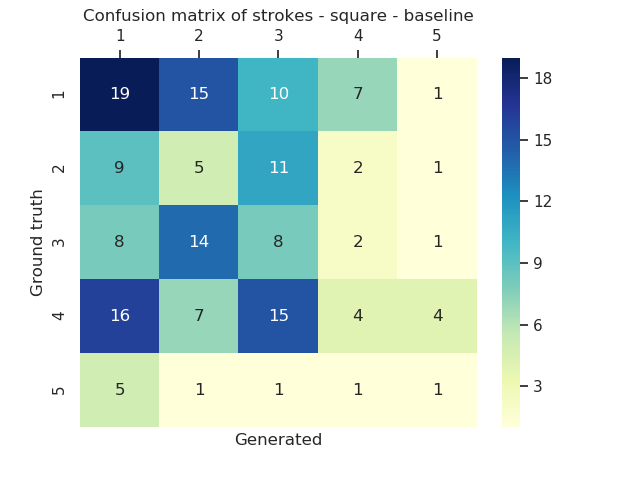
\includegraphics[width=\textwidth]{images/sota/quickdraw_results/quickdraw_square_target_strokes_heatmap.png}
        \end{subfigure}
        ~
        \begin{subfigure}[tb]{0.45\textwidth}
            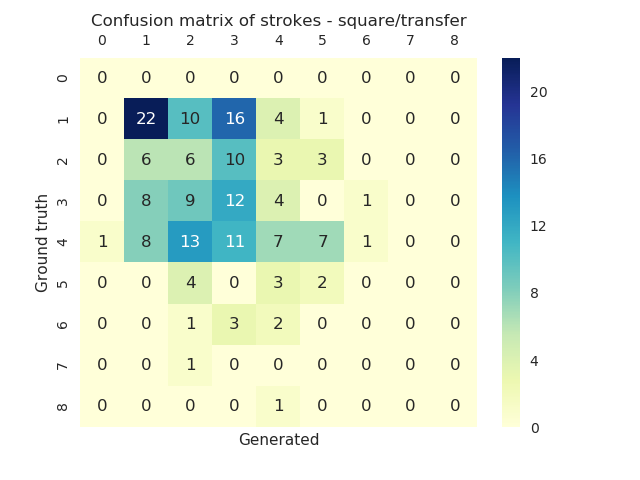
\includegraphics[width=\textwidth]{images/sota/quickdraw_results/quickdraw_square_transfer_strokes_heatmap.png}
        \end{subfigure}

      \end{figure}
      \begin{figure}\ContinuedFloat

        \begin{subfigure}[tb]{0.45\textwidth}
            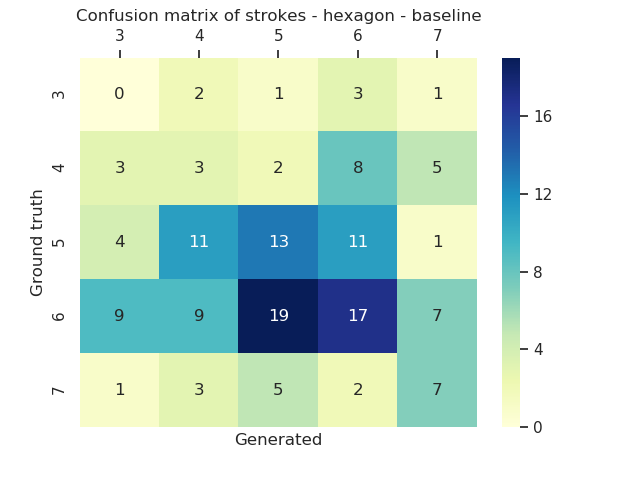
\includegraphics[width=\textwidth]{images/sota/quickdraw_results/quickdraw_hexagon_target_strokes_heatmap.png}
        \end{subfigure}
        ~
        \begin{subfigure}[tb]{0.45\textwidth}
            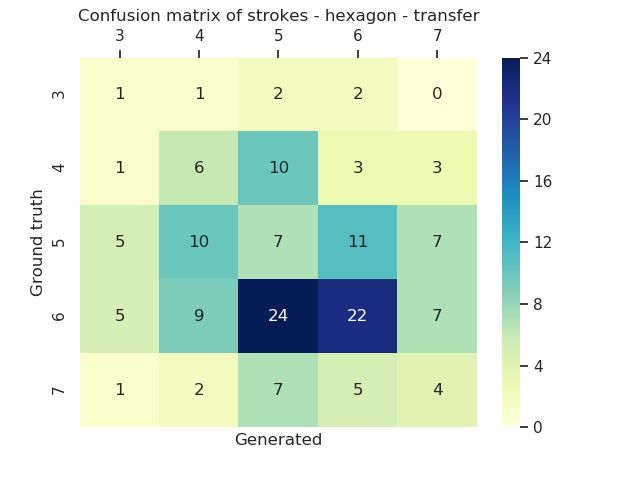
\includegraphics[width=\textwidth]{images/sota/quickdraw_results/quickdraw_hexagon_transfer_strokes_heatmap.png}
        \end{subfigure}

        ~
        \begin{subfigure}[tb]{0.45\textwidth}
            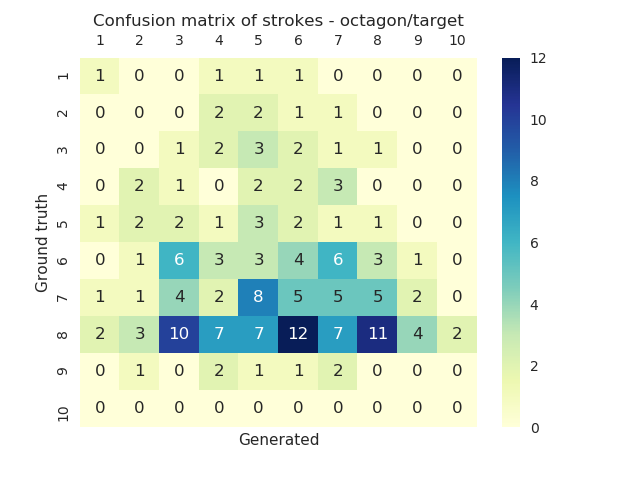
\includegraphics[width=\textwidth]{images/sota/quickdraw_results/quickdraw_octagon_target_strokes_heatmap.png}
        \end{subfigure}
        ~
        \begin{subfigure}[tb]{0.45\textwidth}
            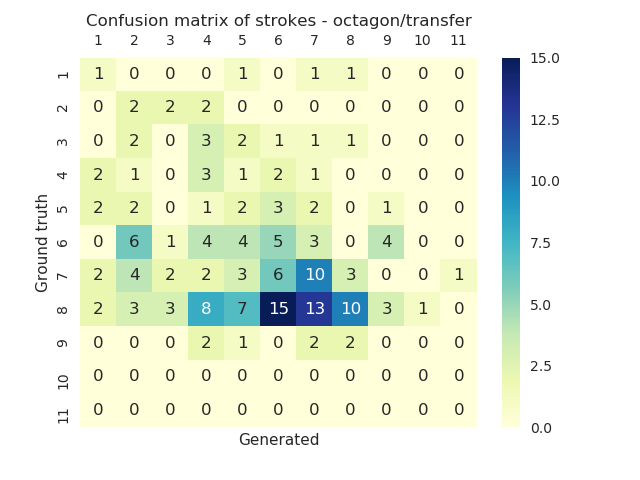
\includegraphics[width=\textwidth]{images/sota/quickdraw_results/quickdraw_octagon_transfer_strokes_heatmap.png}
        \end{subfigure}

        \caption{QuickDraw! Confusion matrix for strokes for both baseline and transfer modes, on the different tasks.}
        \label{fig:quickdraw_strokes_cnf}
      \end{figure}


\section{Style Extraction}

\section{Summary}
